% Don't include figurelist and tablelist,
% otherwise pdflatex can't compile twice causing crossrefs not working
\documentclass[subfigure, nofigurelist, notablelist]{uofsthesis-cs}
\usepackage{amsmath, amssymb, amsthm}
\usepackage{physics}
\usepackage{float, subcaption, graphicx}

\theoremstyle{plain}
\newtheorem{proposition}{Proposition}

\theoremstyle{definition}
\newtheorem{definition}{Definition}

\newtheorem{theorem}{Theorem}
% Documentation for the uofsthesis-cs class is given in uofsthesis-cs.dvi
% 
% It is recommended that you read the CGSR thesis preparation
% guidelines before proceeding.
% They can be found at http://www.usask.ca/cgsr/thesis/index.htm

%%%%%%%%%%%%%%%%%%%%%%%%%%%%%%%%%%%%%%%%%%%%%%%%%%%%%%%%%%%%%%%%%%%%%%%%%%%%%%
% FRONTMATTER - In this section, specify information to be used to
% typeset the thesis frontmatter.
%%%%%%%%%%%%%%%%%%%%%%%%%%%%%%%%%%%%%%%%%%%%%%%%%%%%%%%%%%%%%%%%%%%%%%%%%%%%%%

\title{Instability In Magnetic Nozzle and Spectral Pollution}
\author{Hunt Feng}
\degree{\MSc}

% THESIS DEFENCE DATE
% Should be month year, e.g. July 2004
\defencedate{Month Year}
\department{Physics and Engineering Physics}
% PERMISSION TO USE ADDRESS
\ptuaddress{Head of the Department of Physics and Engineering Physics\\
University of Saskatchewan\\
116 Science Place, Rm 163\\
Saskatoon, SK S7N 5E2\\
Canada
}

% ABSTRACT
\abstract{
This is the abstract of my thesis.  
}

% THESIS ACKNOWLEDGEMENTS -- This can be free-form.
\acknowledgements{
    I would like to express my deepest appreciation to my professor, Andrei Smolyakov. I am also grateful to the former student of my professor, Ivan Khalzov.
}

% THESIS DEDICATION -- Also free-form.  If you don't want a dedication, comment out the following
% line.
\dedication{To my wife and my parents.}

% LIST OF ABBREVIATIONS - Sample  
% If you don't want a list of abbreviations, comment the following 4 lines.
% \loa{
% \abbrev{SCUBA}{Self Contained Underwater Breathing Apparatus\hfill}
% \abbrev{LOF}{List of Figures}
% \abbrev{LOT}{List of Tables}
% }

%%%%%%%%%%%%%%%%%%%%%%%%%%%%%%%%%%%%%%%%%%%%%%%%%%%%%%%%%%%%%%%%
% END OF FRONTMATTER SECTION
%%%%%%%%%%%%%%%%%%%%%%%%%%%%%%%%%%%%%%%%%%%%%%%%%%%%%%%%%%%%%%%%
\begin{document}
% Typeset the title page
\maketitle
\tracingall

% Typeset the frontmatter.  
\frontmatter

%%%%%%%%%%%%%%%%%%%%%%%%%%%%%%%%%%%%%%%%%%%%%%%%%%%%%%%%%%%%%%%%
% FIRST CHAPTER OF THESIS BEGINS HERE
%%%%%%%%%%%%%%%%%%%%%%%%%%%%%%%%%%%%%%%%%%%%%%%%%%%%%%%%%%%%%%%%
\chapter{Introduction}
\section{Motivation}
With the depletion of the earth's resources, the development of space has become a topic that cannot be avoided for mankind. To make space development possible, the necessary space propulsion technology must progress. 

To understand the advantage of electric propulsion. We need to review how propulsion system works. In order to change momentum, a spacecraft needs to expel parts of its mass, the propellant. The motion can be fully characterized by the Newton's second law.
\[ \dv{(mv_e)}{t} = \dot{m}v_e \]
where $m$ is the propellant mass, and $v_e$ is the exhaust velocity.

In 1903, a Russian and soviet rocket scientist, Konstantin Tsiolkovsky, derived the famous rocket equation that relates the change of a rocket's velocity to its exhaust velocity, and the mass of the rocket and propellant,
\[ \Delta v = -v_e \ln(\frac{M}{M+m}) \]
where $\delta v$ is the change in velocity of the spacecraft, $M$ is the mass of spacecraft without propellant, and $m$ is the mass of propellant.

From the Tsiolkovsky rocket equation, we see that higher the ratio between empty rocket and fueled rocket, higher the final velocity. Moreover, if the mass ratio is fixed, then a high exhaust velocity is needed in order to achieve higher final speed. In a chemical rocket, the exhaust velocity of propellant is limited by the temperature of the combustion fuels.

\begin{figure}[H]
	\centering
	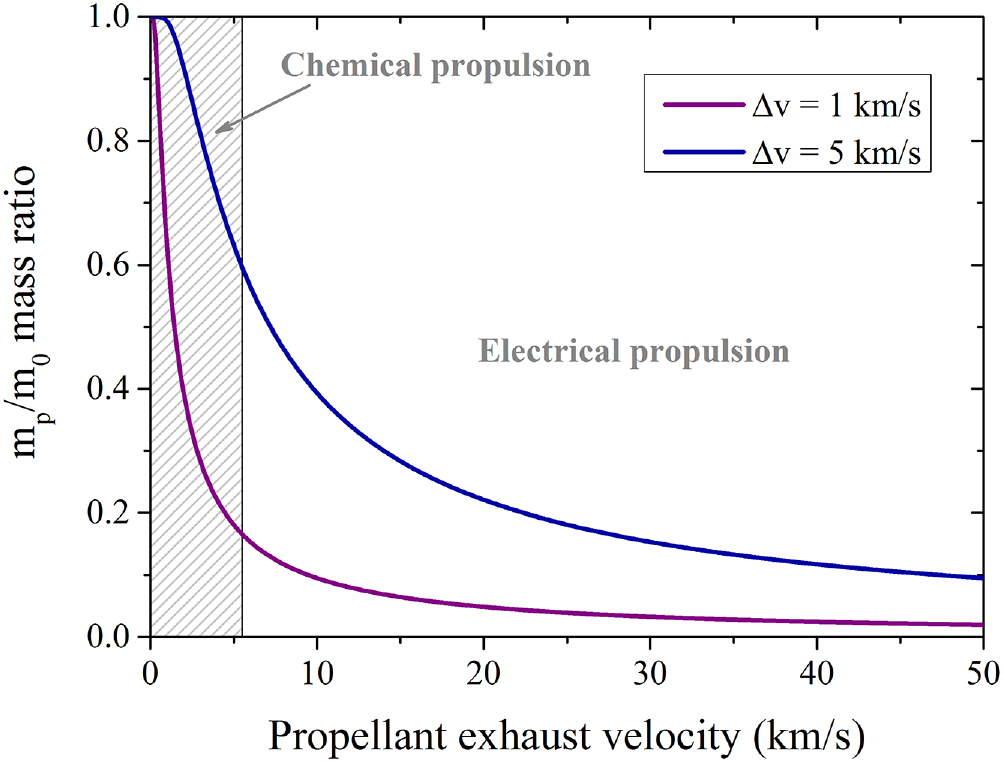
\includegraphics[width=0.7\linewidth]{img/introduction/mass_ratio_vs_exhaust_velocity}
	\caption{Ratio of the propellant mass to the initial mass as a function of the exhaust velocity ve for two values of the velocity increment $\Delta v$ . The dashed area corresponds to the domain of chemical propulsion with ve below 5.5 $km \, s^{-1}$. \cite{mazouffre_electric_2016} }
	\label{fig:massratiovsexhaustvelocity}
\end{figure}



\section{Magnetic Nozzle}
Magnetic nozzle is a convergent-divergent magnetic field that guides, expands and accelerates a plasma jet into vacuum for the purpose of space propulsion. \cite{andersen_continuous_1969,boswell_experimental_2004,williams_fusion_2003} The configuration is of the magnetic field in the magnetic nozzle plays a similar role to the walls of a Laval nozzle, see Fig. \ref{fig:magnetic-nozzle}. The plasma flow starts from subsonic at one end can be accelerated to supersonic at the other end. 

One advantage of magnetic nozzle is that it can operate contactlessly. Since the magnetic nozzle converts the plasma thermal energy into kinetic energy, so the thrust and specific impulse are strongly dependent on the temperature of the plasma flow. Higher the plasma temperature, more effective the plasma thruster. The magnetic field in the magnetic nozzle bounds the hot plasma, and therefore prevents the contact of the nozzle wall and the hot plasma jet. Hence, magnetic nozzle is an appealing plasma acceleration technology. Fig. \ref{fig:massratiovsexhaustvelocity} shows the comparison between magnetic nozzle and traditional chemical rocket.

Moreover, the configuration of magnetic field in magnetic nozzle is important for many other applications,\cite{smolyakov_quasineutral_2021} such as the magnetic divertors in fusion devices,\cite{ryutov_divertor_2016,togo_characteristics_2019} and is also related to the solar wind and accretion flow.\cite{jockers_stability_1968,aikawa_stability_1979} 

\begin{figure}[H]
	\centering
	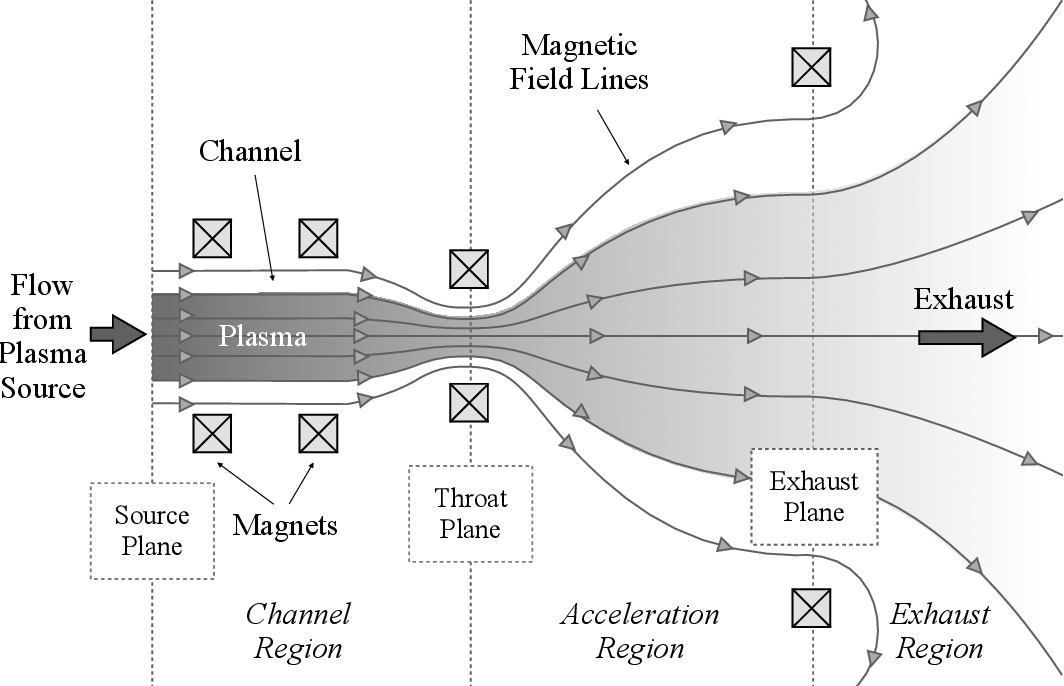
\includegraphics[width=0.7\linewidth]{img/introduction/magnetic_nozzle}
	\caption{Example of a magnetic nozzle configuration. In our models, we define the magnetic nozzle as the region downstream from the throat plane, which can be further divided into an acceleration region and exhaust region. The channel connects the plasma source (not shown) with the magnetic nozzle. \cite{little_performance_2015}}
	\label{fig:magnetic-nozzle}
\end{figure}


\section{Plasma Instability}
However, the plasma motion is determined by the Lorentz force, the nature of the nonlinearity of the motion makes it hard to predict analytically. Since the construction of Tokamak, people underestimated the difficulty of describing plasma motion. Hence, in order to maintain the equilibrium in the Tokamak, people start analyzing the stability of plasma. Nowadays, the study of plasma instabilities is an important area in plasma physics. 

Consider a plasma system in at equilibrium, we introduce a small perturbation to it. The stability of the system determines if the perturbations will grow, oscillate, or be damped out. Similar to the study of mechanical stability at equilibrium. See Fig. \ref{fig:stability-visualization}.

\begin{figure}[H]
	\centering
	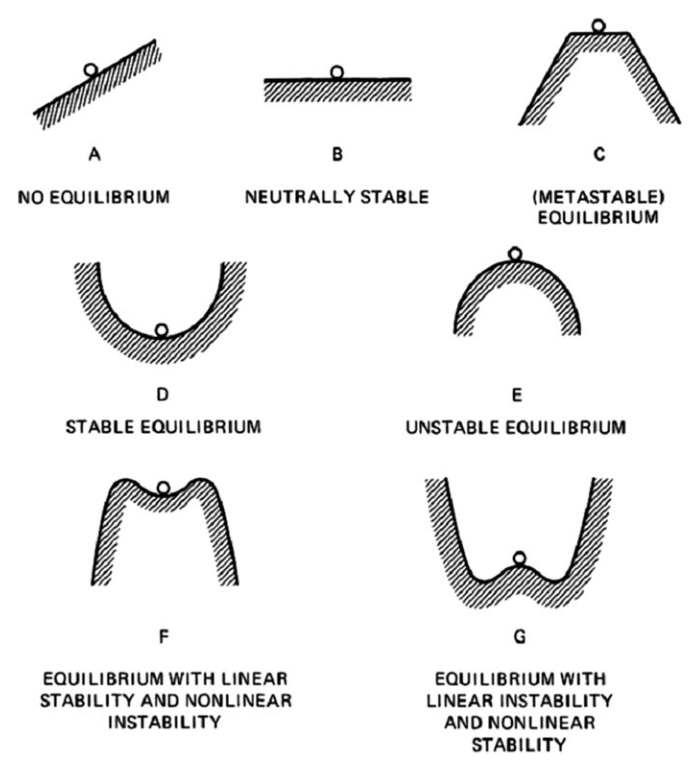
\includegraphics[width=0.7\linewidth]{img/introduction/stability_visualization}
	\caption{Mechanical analogy of various types of equilibrium. \cite{chen_introduction_2016}}
	\label{fig:stability-visualization}
\end{figure}


\subsection{Illustration: Two-Stream Instability}
We take the famous two-stream instability as an illustration. Let the plasma be cold ($k_BT_e = k_BT_i = 0$), let there be no magnetic field ($B_0=0$). The linearized continuity equations are
\begin{align} 
	\pdv{n_{i1}}{t} + n_0\pdv{v_{i1}}{x} &= 0  \label{eq:two-stream-continuity1} \\
	\pdv{n_{e1}}{t} + n_0\pdv{v_{e1}}{x} + v0\pdv{n_{e1}}{x} &= 0 \label{eq:two-stream-continuity2}
\end{align}

And the linearized equations of motion are
\begin{align} 
	Mn_0\pdv{v_{i1}}{t} &= en_0E_1  \label{eq:two-stream-eom1} \\
	mn_0\left(\pdv{v_{e1}}{t} + v_0\pdv{v_{e1}}{x}\right) &= -en_0E_1 \label{eq:two-stream-eom2}
\end{align}
Here $v_0$ is the velocity of electron respect to the ions (the ion velocity at equilibrium is taken to be $v_{i0}=0$), $n_0$ is the equilibrium density of both ion and electron, $v_{i1}$ and $v_{e1}$ are perturbed velocity of ions and electrons, and $E_1$ is the perturbed electron field.

If we assume perturbed electric field takes the wave form
\[ E_1 = E\exp(i(kx-\omega t)) \]
Plug this perturbed electric field into Eq.(\ref{eq:two-stream-eom1}) and (\ref{eq:two-stream-eom2}), then we can solve for $v_{i1}$ and $v_{e1}$,
\begin{align*}
	v_{i1} &= \frac{ie}{M\omega} E \\
	v_{e1} &= -\frac{ie}{m}\frac{E}{\omega-kv_0}
\end{align*}

Using the perturbed velocities, the continuity equations Eq.(\ref{eq:two-stream-continuity1}) and (\ref{eq:two-stream-continuity2}) yields
\begin{align*}
	n_{i1} &= \frac{ien_0k}{M\omega^2} E \\
	n_{e1} &= \frac{iekn_0}{m(\omega-kv_0)^2}E
\end{align*}

Finally, plug them into the Poisson's equation
\[ \epsilon_0 \pdv{E_1}{x} = e(n_{i1}-n_{e1}) \]
We now have the dispersion relation
\[ 1 = \omega_p \left[\frac{m/M}{\omega^2}+\frac{1}{(\omega-kv_0)^2}\right] \]

Solving this equation for $\omega$, there is chance we will get complex frequency,
\[ \omega = \omega_r + i\omega_i \]
where $\omega_r, \omega_i \in\mathbb{R}$. Then the perturbed electric field becomes
\[ E_1 = E\exp(i(kx-\omega_rt))\exp(\omega_it) \]

When $\omega_i < 0$, it is a damped wave, when $\omega_i > 0$, it grows exponentially and therefore unstable. Since the complex root comes with pair, as long as $\omega_i\neq 0$, one of the roots must correspond to an unstable wave. The following graph shows the two-stream instability in phase space.

\begin{figure}[H]
	\centering
	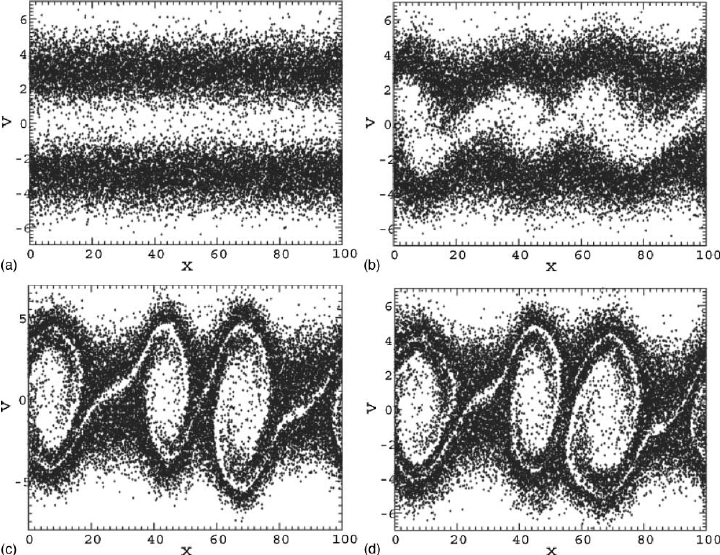
\includegraphics[width=0.7\linewidth]{img/introduction/two_stream_instability}
	\caption{Visualization of two-stream instability in the phase space. (a) Initially the ion and electron flow are in opposite direction. (b) The velocity of both flows start to oscillate. (c) Chaotic behavior occurs. (d) The chaotic behavior continues. \cite{ha_nonlinear_2011}}
	\label{fig:two_stream_instability}
\end{figure}

\subsection{Stability of Configurations Similar to Magnetic Nozzle}
Accretion flow has configuration similar to the magnetic nozzle. It is natural to find studies of stability the accretion flow. However, the results are still debatable. \cite{keto_stability_2020,aikawa_stability_1979,stellingwerf_stability_1978}


\section{Goals of this Thesis}
The goals of this thesis is to first study the spectral method for solving the instability problem. When using the spectral method, it is necessary to understand different discretizations of the operators, such as finite difference, finite element and DVR method.

Once the spectral method is introduced, we can use it to study the instability of plasma in magnetic nozzle. We can use different discretization techniques, and compare the results from different methods.

Finally, we need to take care of the filtering of the spectral pollution.


\section{Thesis Outline}
The theory of spectral methods will be discussed in chapter \ref{chap:spectral_method}. In this chapter, different discretiation methods will be introduced. Moreover, a very important concept, spectral pollution, will be introduced in detailed in the final section of this chapter.

Then, in chapter \ref{chap:governing_equations} is the discussion of governing equations and its linearization. The formulation of the problem will be derived in this chapter.

In chapter ??, we ill use the equations derived in chapter \ref{chap:governing_equations} to conduct numerical experiments. The goal is to investigate the frequency of each modes. The filtering methods of spurious modes will be introduced.

Conclusion will in chapter ??


\section{Spectral Method}
\begin{frame}{Spectral Method}
  Eq.(\ref{eq:polynomial_eigenvalue_problem}) can be reformulate as 
  \begin{equation} \label{eq:eigenvalue-problem}
	\mqty[ 0 & 1\\ \hat{M} & \hat{N} ]\mqty[ \tilde{v}\\ \omega \tilde{v}] = \omega\mqty[ \tilde{v}\\ \omega \tilde{v}]
\end{equation}
where the operators $\hat{M}$ and $\hat{N}$ are defined as
\begin{align*}
	\hat{M} = &-\left[(1-v_0^2)\pdv[2]{}{z} 
	-\left(3v_0 + \frac{1}{v_0}\right)\pdv{v_0}{z}\pdv{}{z}\right. \\ 
  &- \left.  \left(1-\frac{1}{v_0^2}\right)\left(\pdv{v_0}{z}\right)^2 
	- \left(v_0+\frac{1}{v_0}\right)\pdv[2]{v_0}{z}\right] \\
	\hat{N} = &-2i\left(v_0\pdv{}{z} +\pdv{v_0}{z} \right) 
\end{align*}
  Then by discretizing operators $\hat{M},\hat{N}$, this becomes an algebraic eigenvalue problem.
\end{frame}

\begin{frame}{Spectral Pollution}
  \begin{itemize}
    \item All modes of Eq.(\ref{eq:polynomial_eigenvalue_problem}) with $v_0=\text{const}$ are stable.
    \item Yet all discretization show unstable modes.
  \end{itemize}
  \begin{figure}[htbp]	
    \centering
    \begin{subfigure}[b]{0.5\linewidth}
      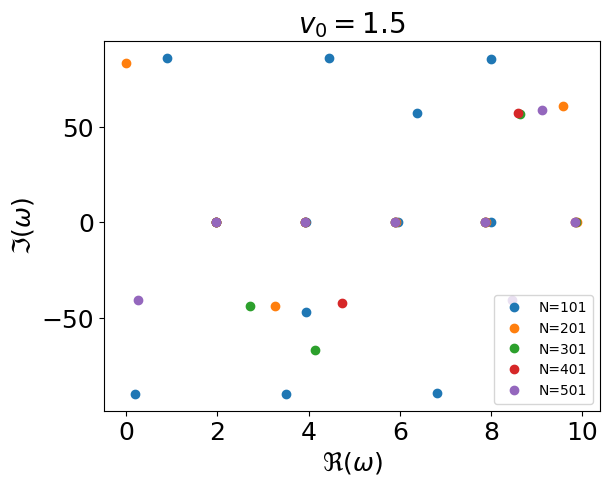
\includegraphics[width=0.9\linewidth]{figures/eigvals-bad} 
      \caption{Unfiltered eigenvalues.}
    \end{subfigure}%
    \begin{subfigure}[b]{0.5\linewidth}
      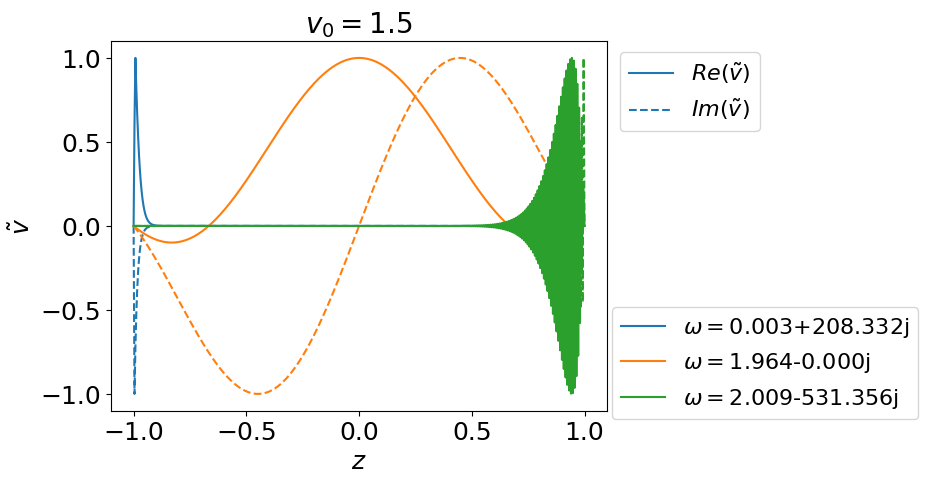
\includegraphics[width=0.9\linewidth]{figures/eigvecs-bad} 
      \caption{First few unfiltered eigenfunctions.}
    \end{subfigure}
    \caption{Finite difference discretization was used. Spurious modes occurs regardless of the resolution.}
    \label{fig:results-bad}
  \end{figure}
\end{frame}

\begin{frame}{Filtering Spurious Modes}
  \begin{figure}[htbp]
    \centering
    \begin{subfigure}[b]{0.5\linewidth}
      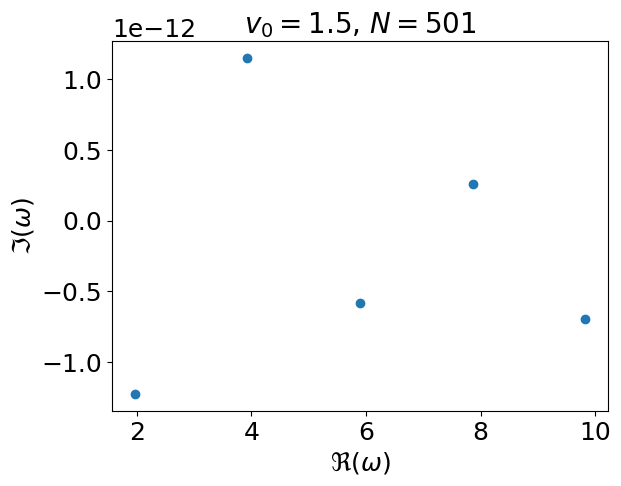
\includegraphics[width=\linewidth]{figures/eigvals-good} 
      \caption{Filtered eigenvalues.}
    \end{subfigure}%
    \begin{subfigure}[b]{0.5\linewidth}
      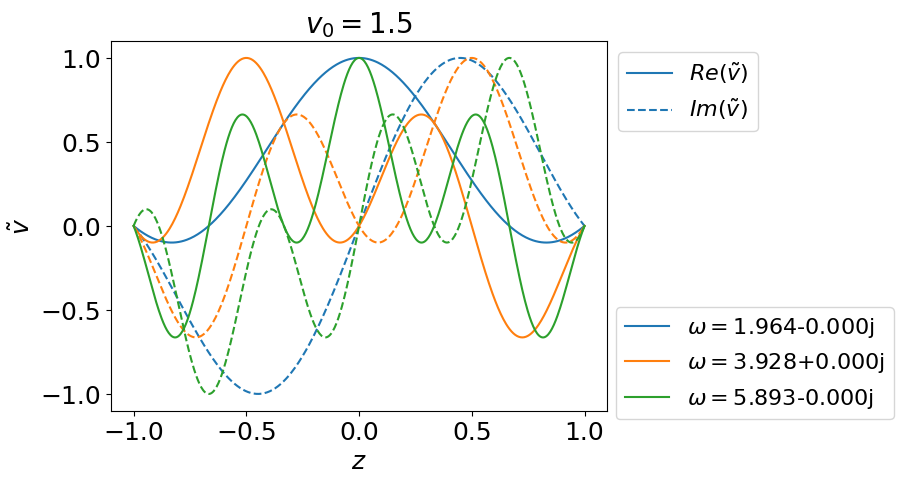
\includegraphics[width=\linewidth]{figures/eigvecs-good} 
      \caption{First few filtered eigenfunctions.}
    \end{subfigure}
    \caption{The spurious modes are changing under different resolution. We can filter them by convergence test.}
    \label{fig:results-good}
  \end{figure}
\end{frame}

\chapter{Equations Of Motion}
The dynamics of magnetic nozzle can be characterized by conservation of mass and momentum,
\begin{align*}
    &\pdv{n}{t} + B\pdv{z}(\frac{nv}{B}) = 0\\
    &\pdv{v}{t} + v\pdv{v}{z} = -c_s^2\frac{1}{n}\pdv{n}{z}
\end{align*}
Usually, the magnetic field can be described by
\[ B(z) = B_0\left[ 1 + R\exp(-\frac{z^2}{\delta^2}) \right] \]
where $R$ and $\delta$ are some coefficients.

At equilibrium (stationary solution), we have $\pdv*{n_0}{t}=0$ and $\pdv*{v_0}{t}=0$, so $n_0$ and $v_0$ satisfy
\begin{align*}
    &\pdv{z}(\frac{n_0v_0}{B}) = 0 \\
    &v_0\pdv{v_0}{z} = -c_s^2\frac{1}{n_0}\pdv{n_0}{z} 
\end{align*}
Let $M\equiv v_0/c_s$, then it can be represented by Lambert function, 
\[ M = \left[ -W\left(-M_m^2 \frac{B(z)^2}{B_m^2}e^{-M_m^2}\right) \right]^{1/2} \]
where $B_m\equiv 1+R$ is the maximum magnetic field (or magnetic field at mid-point), and $M_m$ is the mach number at mid-point. Below shows a few cases of the solution.
\begin{itemize}
    \item $M_m < 1$, subsonic velocity profile.
    \item $M_m = 1$, accelerating or decelerating profile (depending on the branch of the Lambert function).
    \item $M_m > 1$, supersonic velocity profile
\end{itemize}
\begin{figure}[H]
    \centering
    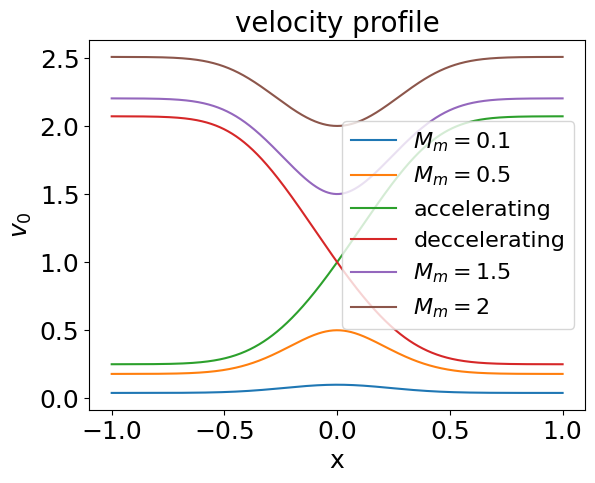
\includegraphics[width=0.7\linewidth]{img/nozzle-velocity-profile.png}
    \caption{$M_m < 1$, subsonic. $M_m = 1$, accelerating if we select Lambert function branch $k=0$ for $z<0$ and brach $k=-1$ for $z>=0$; decelerating if we choose branch $k=-1$ for $z<0$ and brach $k=0$ for $z>=0$. $M_m > 1$, supersonic.}
    \label{fig:nozzle-velocity-profile}
\end{figure}

For convenience, we nondimensionalize the equations by normalizing the velocity to $c_s$, $v\mapsto v/c_s$, $z$ to system length $L$, $z \mapsto z/L$ and time $t\mapsto c_s t/L$.
\begin{align}
    &\pdv{n}{t} + n\pdv{v}{z} + v\pdv{n}{z} - nv\frac{\partial_z B}{B} = 0 \\
    &n\pdv{v}{t} + nv\pdv{v}{z} = -\pdv{n}{z}
\end{align}
and the nondimensionalized equilibrium condition is
\begin{align}
    &\pdv{z}(\frac{n_0v_0}{B}) = 0 \label{eq:equilibrium-convervation-of-mass}\\
    &v_0\pdv{v_0}{z} = -\frac{1}{n_0}\pdv{n_0}{z} \label{eq:equilibrium-convervation-of-momentum}
\end{align}


\begin{proposition}
    Let $n = n_0(z) + \tilde{n}(z,t)$ and $v = v_0(z) + \tilde{v}(z,t)$, the linearized equations of motion are
    \begin{align}
        &\frac{1}{n_0}\pdv{\tilde{n}}{t} 
        + \pdv{\tilde{v}}{z} + v_0\tilde{Y} + \tilde{v}\frac{\partial_z n_0}{n_0} - \tilde{v}\frac{\partial_z B}{B} = 0 
        \label{eq:linearized-conservation-of-mass}
        \\
        &\pdv{\tilde{v}}{t} + \pdv{(v_0\tilde{v})}{z} = -\tilde{Y}
        \label{eq:linearized-conservation-of-momentum}
    \end{align}
    where 
    \[ \tilde{Y} \equiv \frac{1}{n_0}\pdv{\tilde{n}}{z} - \frac{\partial_z n_0}{n_0^2}\tilde{n} = \pdv{z}(\frac{\tilde{n}}{n_0}) \]
\end{proposition}
\begin{proof}
    We first derive Eq.(\ref{eq:linearized-conservation-of-mass}). We linearize Eq.(\ref{eq:equilibrium-convervation-of-mass}) by setting $n=n_0+\tilde{n}$ and $v=v_0+\tilde{v}$. By ignoring the second order perturbations, we obtain
    \begin{align*}
        &\pdv{(n_0+\tilde{n})}{t} 
        + (n_0+\tilde{n})\pdv{(v_0+\tilde{v})}{z} 
        + (v_0+\tilde{v})\pdv{(n_0+\tilde{n})}{z} 
        - (n_0+\tilde{n})(v_0+\tilde{v})\frac{\partial_z B}{B} = 0 \\
        \Rightarrow 
        &\pdv{\tilde{n}}{t} 
        + n_0\pdv{v_0}{z} + \tilde{n}\pdv{v_0}{z} + n_0\pdv{\tilde{v}}{z}
        + v_0\pdv{n_0}{z} + \tilde{v}\pdv{n_0}{z} + v_0\pdv{\tilde{n}}{z} 
        - (n_0v_0 + n_0\tilde{v} + \tilde{n}v_0)\frac{\partial_z B}{B} = 0 \\
        \Rightarrow
        &\frac{1}{n_0}\pdv{\tilde{n}}{t} 
        + \pdv{v_0}{z} + \frac{\tilde{n}}{n_0}\pdv{v_0}{z} + \pdv{\tilde{v}}{z}
        + \frac{v_0}{n_0}\pdv{n_0}{z} + \frac{\tilde{v}}{n_0}\pdv{n_0}{z} + \frac{v_0}{n_0}\pdv{\tilde{n}}{z} 
        - v_0\frac{\partial_z B}{B} - \tilde{v}\frac{\partial_z B}{B} - \tilde{n}\frac{v_0}{n_0}\frac{\partial_z B}{B} = 0
    \end{align*}
    Using the equilibrium condition Eq.(\ref{eq:equilibrium-convervation-of-mass}), some of the terms are canceled and the last term can be written as 
    \[ \tilde{n}\frac{v_0}{n_0}\frac{\partial_z B}{B} = \frac{\tilde{n}}{n_0}\left( \frac{\partial_z n_0}{n_0}v_0 + \pdv{v_0}{z} \right) \]
    Now, we are left with equation
    \[
        \frac{1}{n_0}\pdv{\tilde{n}}{t}
        + \pdv{\tilde{v}}{z}
        + v_0\underbrace{\left(\frac{1}{n_0}\pdv{\tilde{n}}{z} - \frac{\tilde{n}}{n_0}\frac{\partial_z n_0}{n_0}  \right)}_{\tilde{Y}}
        + \frac{\tilde{v}}{n_0}\pdv{n_0}{z}
        - \tilde{v}\frac{\partial_z B}{B} = 0
    \]

    To derive Eq.(\ref{eq:linearized-conservation-of-momentum}), we linearize the LHS of the conservation of momemtum
    \begin{align*}
        &(n_0+\tilde{n})\pdv{(v_0+\tilde{v})}{t} + (n_0+\tilde{n})(v_0+\tilde{v})\pdv{(v_0+\tilde{v})}{z} = -\pdv{n}{z} \\
        \Rightarrow 
        & \pdv{v_0}{t} + \frac{\tilde{n}}{n_0}\pdv{v_0}{t} + \pdv{\tilde{v}}{t} 
        + \left(v_0+\tilde{v}+\frac{\tilde{n}}{n_0}v_0\right)\pdv{(v_0+\tilde{v})}{z} = -\frac{1}{n_0}\pdv{n}{z}\\
        \Rightarrow
        & \pdv{v_0}{t} + v_0\pdv{v_0}{z} + \tilde{v}\pdv{v_0}{z} 
        = -\frac{1}{n_0}\pdv{n_0}{z} -\frac{1}{n_0}\pdv{\tilde{n}}{z} -v_0\frac{v_0}{z} - \frac{\tilde{n}}{n_0}v_0\pdv{v_0}{z} \\ 
    \end{align*}
    Using the equilibrium condition Eq.(\ref{eq:equilibrium-convervation-of-momentum}) on the RHS, we get the desired form.
\end{proof}

\[ \int fdx = 1 \]

\cite{stellingwerf_stability_1978}
\chapter{Numerical Experiments}
In this chapter, we will solve the eigenvalue problem, Eq.(\ref{eq:eigenvalue-problem}), with different discretizations. There will be three major categories of methods used. Finite difference (FD) method, finite element (FE) method and spectral element method (SE).

The finite difference method will be used together with equally spaced nodes. The finite element method will use B-spline as basis functions. Finally, the spectral element method uses sine functions as the spectral elements.

For Dirichlet boundary, The parameters of different discretizations are listed below
\begin{table} [H]
	\centering
	\caption{With Dirichlet boundary condition, all methods have good accuracy, so using 101 nodes in the region $[0,1]$ is enough. For FE and SE methods, they are using ~50 basis functions.}
	\begin{tabular}{|c|c|c|c|}
		\hline
		& FD & FE\_BSPLINE & SE\_SINE  \\
		\hline
		N & 101 & 101 & 101 \\
		\hline
		NUM\_BASIS &  & 51 & 50 \\
		\hline
	\end{tabular}
	\label{table:parameters-dirichlet}
\end{table}

For left-fixed and right-open (fixed-open) boundary condition, the parameters are    
\begin{table} [H]
	\centering
	\caption{With fixed-open boundary condition, it requires higher resolution in order to get accurate results. Therefore all methods use 501 nodes in the region $[0,1]$, and FE method uses 101 basis functions.}
	\begin{tabular}{|c|c|c|}
		\hline
		& FD & FE\_BSPLINE \\
		\hline
		N & 501 & 501 \\
		\hline
		NUM\_BASIS &  & 101 \\
		\hline
	\end{tabular}
	\label{table:parameters-fixed-open}
\end{table}


\section{Constant Velocity Case}
\subsection{Dirichlet Boundary}
Because the existence of exact solution to problems Eq.(\ref{eq:constant-v-problem-dirichlet}). The case with constant velocity profile is used as a sanity check. It allows us to verify the correctness of each method's implementation. This also serves as a reference to the accuracy spectral methods can achieve.

From Fig.(\ref{fig:constant-v}), we see that the order of growth rates obtained by different methods is about $~10^{-14}$ for both subsonic and supersonic cases. We will use these numbers as a reference to the accuracy of our numerical methods. If a method produces growth rates with order close to $10^{-14}$, we consider the growth rates to be 0.

\begin{table} [H]
	\centering
	\caption{Relative error of each eigenvalue.}
	\begin{tabular}{|c|c|c|c|c|c|}
		\hline
		$v_0=0.5$   & 1 & 2 & 3 & 4 & 5 \\
		\hline
		FD & 2.827e-05 & 1.130e-04 & 2.541e-04 & 4.512e-04 & 7.040e-04 \\
		\hline
		FE & 0.005 & 0.005 & 0.006 & 0.008 & 0.010  \\
		\hline
		SE & 2.896e-05 & 1.157e-04 & 2.603e-04 & 4.626e-04 & 7.217e-04 \\
		\hline
	\end{tabular}
	\begin{tabular}{|c|c|c|c|c|c|}
		\hline
		$v_0=1.5$   & 1 & 2 & 3 & 4 & 5 \\
		\hline
		FD & 0.001 & 0.005 & 0.010 & 0.019 & 0.030 \\
		\hline
		FE & 0.006 & 0.010 & 0.019 & 0.029 & 0.043  \\
		\hline
		SE & 0.001 & 0.005 & 0.011 & 0.019 & 0.030 \\
		\hline
	\end{tabular}
	\label{table:eigenvalue-error-dirichlet}
\end{table}

\begin{figure}[H]
	\centering
	\begin{subfigure}{0.5\textwidth}
		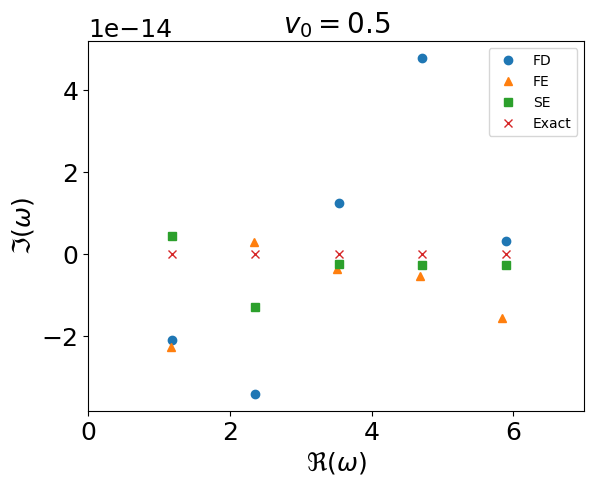
\includegraphics[width=\linewidth]{../../thesis/img/numerical-experiments/fixed-fixed/constant-v-v0=0.5}
		\caption{All modes are stable.}
	\end{subfigure}%
	\begin{subfigure}{0.5\textwidth}
		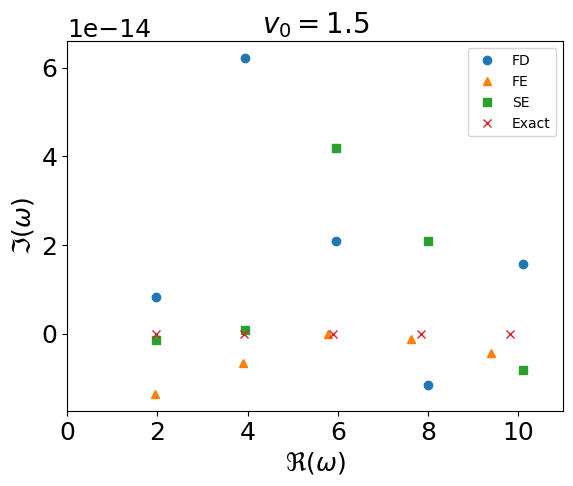
\includegraphics[width=\linewidth]{../../thesis/img/numerical-experiments/fixed-fixed/constant-v-v0=1.5}
		\caption{Filtered modes are stable.}
	\end{subfigure}
	\caption{Showing the first 5 eigenvalues of each method in each case. All methods are close to the exact eigenvalues.}
	\label{fig:constant-v-dirichlet}
\end{figure}

\subsection{Fixed-Open Boundary}
\begin{table} [H]
	\centering
	\caption{Relative error of each eigenvalue. Notice that the ground mode for subsonic case is non-zero.}
	\begin{tabular}{|c|c|c|c|c|c|}
		\hline
		$v_0=0.5$   & 0 & 1 & 2 & 3 & 4 \\
		\hline
		FD & 1.209e-05 & 3.458e-05 & 5.775e-05 & 8.153e-05 & 1.061e-04 \\
		\hline
		FE & 8.090e-05 & 2.007e-04 & 2.981e-04 & 6.596e-04 & 1.821e-03  \\
		\hline
	\end{tabular}
	\begin{tabular}{|c|c|c|c|c|c|}
		\hline
		$v_0=1.5$   & 1 & 2 & 3 & 4 & 5 \\
		\hline
		FD & 9.163e-05 & 2.435e-04 & 4.833e-04 & 8.160e-04 & 1.243e-03 \\
		\hline
		FE & 4.431e-04 & 7.924e-04 & 1.516e-03 & 3.103e-03 & 8.001e-03  \\
		\hline
	\end{tabular}
	\label{table:eigenvalue-error}
\end{table}

\begin{figure}[H]
	\centering
	\begin{subfigure}{0.5\textwidth}
		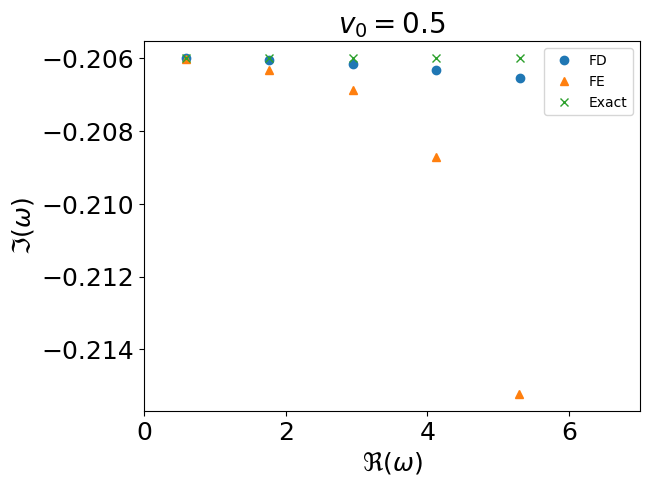
\includegraphics[width=\linewidth]{../../thesis/img/numerical-experiments/fixed-open/constant-v-v0=0.5}
		\caption{All modes are stable.}
	\end{subfigure}%
	\begin{subfigure}{0.5\textwidth}
		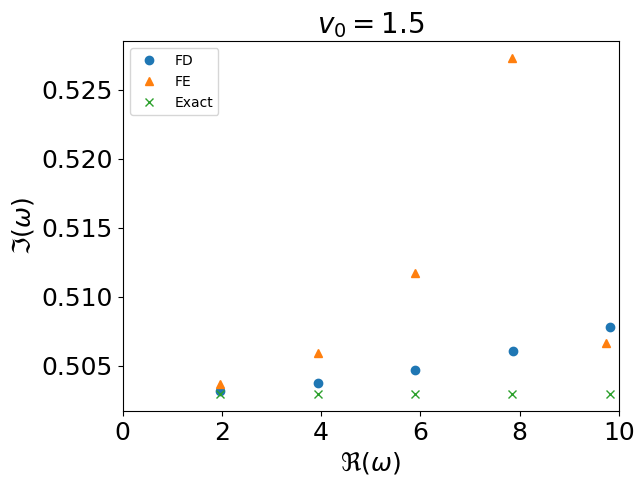
\includegraphics[width=\linewidth]{../../thesis/img/numerical-experiments/fixed-open/constant-v-v0=1.5}
		\caption{All modes are unstable.}
	\end{subfigure}
	\caption{Showing the first 5 eigenvalues of each method. Finite-difference method has much better accuracy than finite-element method.}
	\label{fig:constant-v-fixed-open}
\end{figure}


\section{Subsonic Case}
\subsection{Dirichlet Boundary}
When setting the mid-point velocity to be $M_m=0.5$, we have the subsonic velocity profile. This velocity profile is the orange line shown in Fig.\ref{fig:velocity-profiles}. With Dirichlet boundary condition, $\tilde{v}(\pm 1) =0$. The flow in magnetic nozzle is stable. Fig.\ref{fig:subsonic-v-dirichlet} shows the first few eigenvalues obtained by different discretizations. 

The order of growth rates obtained by different methods is $10^{-13}$, we can consider it to be stable.
\begin{figure} [H]
	\centering
	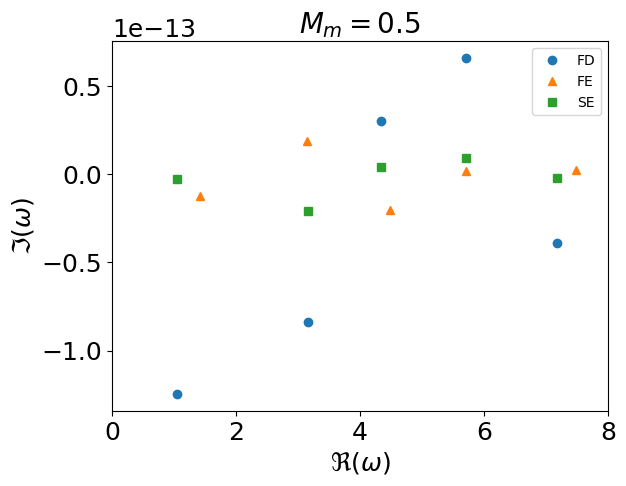
\includegraphics[width=0.7\linewidth]{../../thesis/img/numerical-experiments/fixed-fixed/subsonic-v}
	\caption{Showing the first 5 modes. It suggests that the flow in magnetic nozzle with subsonic velocity profile and Dirichlet boundary condition is stable.}
	\label{fig:subsonic-v-dirichlet}
\end{figure}

\subsection{Fixed-Open Boundary}
\begin{figure} [H]
	\centering
	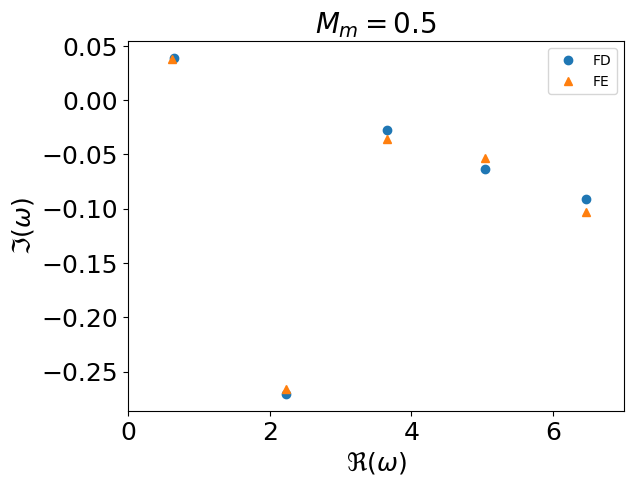
\includegraphics[width=0.7\linewidth]{../../thesis/img/numerical-experiments/fixed-open/subsonic-v}
	\caption{Showing the first 5 modes. The ground mode is unstable, other modes are stable.}
	\label{fig:subsonic-v-fixed_open}
\end{figure}


\section{Supersonic Case}
\subsection{Dirichlet Boundary}
When the velocity profile is supersonic, shown as purple line in Fig.\ref{fig:velocity-profiles}, spurious modes appeared as predicted in Chap.\ref{chap:theoretical-analysis}. Using the convergence test, we successfully eliminates all unstable modes. Fig.(\ref{fig:supersonic-v-dirichlet}) shows the first few filtered eigenvalues. As we can see the flow is stable.
\begin{figure} [H]
	\centering
	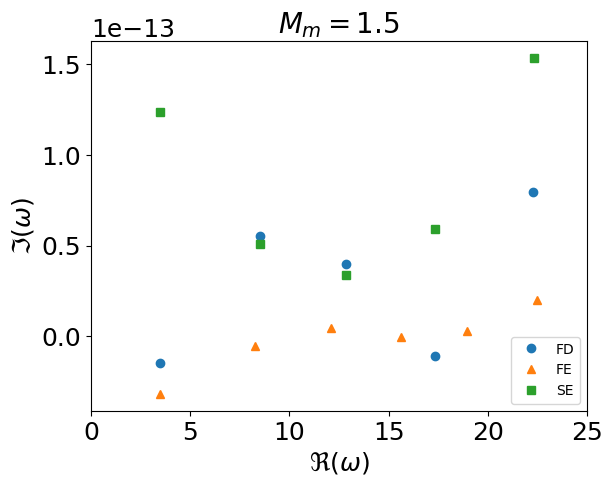
\includegraphics[width=0.7\linewidth]{../../thesis/img/numerical-experiments/fixed-fixed/supersonic-v}
	\caption{First few filtered eigenvalues are shown. The spurious modes are filtered by convergence test.}
	\label{fig:supersonic-v-dirichlet}
\end{figure}

\subsection{Fixed-Open Boundary}
\begin{figure} [H]
	\centering
	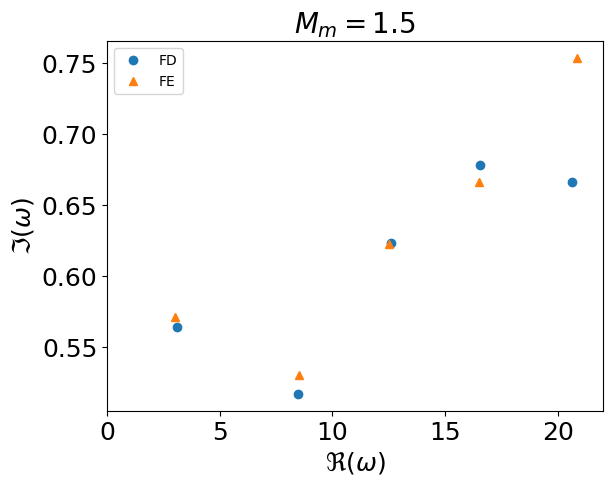
\includegraphics[width=0.7\linewidth]{../../thesis/img/numerical-experiments/fixed-open/supersonic-v}
	\caption{All modes are unstable.}
	\label{fig:supersonic-v-fixed-open}
\end{figure}


\section{Accelerating Case}
Starting from the singular point, we shoot the solution to the left boundary. We find the set of eigenvalues such that $\tilde{v}(-1)=0$. With these eigenvalues, we can extend the solution to the supersonic region $(0,1]$. The first five eigenvalues are drawn in the graph.
\begin{figure} [H]
	\centering
	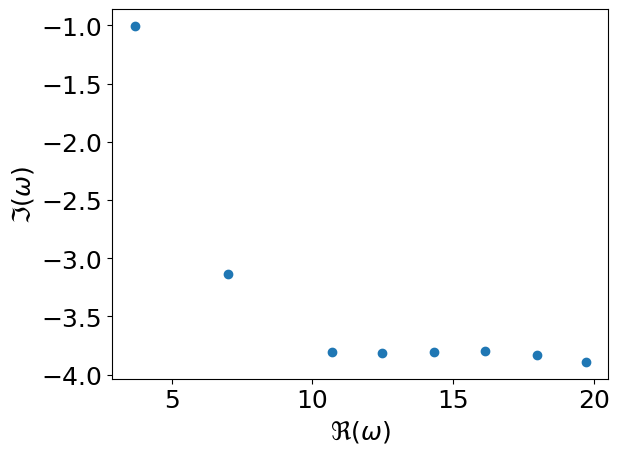
\includegraphics[width=0.7\linewidth]{../../thesis/img/numerical-experiments/accelerating-v}
	\caption{first five modes are stable.}
	\label{fig:accelerating-v}
\end{figure}

% \chapter{conclusion}



%%%%%%%%%%%%%%%%%%%%%%%%%%%%%%%%%%%%%%%%%%%%%%%%%%%%%%%%%%%%%%%%
% The Bibliograpy should go here. BEFORE appendices!
%%%%%%%%%%%%%%%%%%%%%%%%%%%%%%%%%%%%%%%%%%%%%%%%%%%%%%%%%%%%%%%%


% Typeset the Bibliography.  The bibliography style used is "plain".
% Optionally, you can specify the bibliography style to use:
% \uofsbibliography[stylename]{yourbibfile}

\bibliography{references} % this is for intellisence, comment this later

\uofsbibliography{references}

% If you are not using bibtex, comment the line above and uncomment
% the line below.  
%Follow the line below with a thebibliography environmentand bibitems.  
% Note: use of bibtex is usually the preferred method.

%\uofsbibliographynobibtex


%%%%%%%%%%%%%%%%%%%%%%%%%%%%%%%%%%%%%%%%%%%%%%%%%%%%%%%%%%%%%%%%%%%%%%%%%
% APPENDICES
%
% Any chapters appearing after the \appendix command get numbered with
% capital letters starting with appendix 'A'.
% New chapters from here on will be called 'Appendix A', 'Appendix B'
% as opposed to 'Chapter 1', 'Chapter 2', etc.
%%%%%%%%%%%%%%%%%%%%%%%%%%%%%%%%%%%%%%%%%%%%%%%%%%%%%%%%%%%%%%%%%%%%%%%%%%

% Activate thesis appendix mode.
\uofsappendix

% Put appendix chapters in the appendices environment so that they appear correcty
% in the table of contents.  You can use \input's here as well.
\begin{appendices}

\chapter{Sample Appendix}

Stuff for this appendix goes here.

\end{appendices}

\end{document}
